\documentclass[english, 11 pt, class=article, crop=false]{standalone}
\usepackage[T1]{fontenc}
\usepackage[utf8]{luainputenc}
\usepackage{lmodern} % load a font with all the characters
\usepackage{geometry}
\geometry{verbose,a4paper, inner=2.3cm, outer=1.8 cm, bmargin=1cm, tmargin=1cm}
\setlength{\parindent}{0bp}
\usepackage{import}
\usepackage[subpreambles=false]{standalone}
\usepackage{amsmath}
\usepackage{amssymb}
\usepackage{esint}
\usepackage{icomma}
\usepackage{babel}
\usepackage{tabu}
\usepackage[many]{tcolorbox}




\begin{document}
\pagestyle{empty}

{\huge \textbf{Lekseark veke 42}} \\[5pt]

\begin{tcolorbox}[boxrule=0.1 mm,arc=0mm,enhanced jigsaw,breakable,colback=white] {\footnotesize \textbf{Eksempel 1} \\} \footnotesize 
Marker tala $ 0,3 $ og $ 1,7 $ på tallinja.\\[12pt]
\textbf{Svar}
\begin{figure}
	\centering
	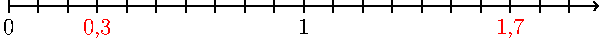
\includegraphics{tallineks}
\end{figure}
 \end{tcolorbox} \vspace{20pt}

\textbf{Oppgåve}

\begin{enumerate}
	\item Marker tala $ 0,9 $ og $ 1,7 $.\\[10pt]	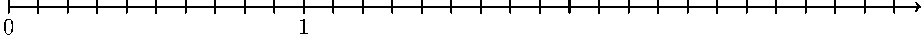
\includegraphics{tallin_0_3}
	\item Marker tala $ 0,1 $ og $ 2,9 $.\\[10pt]	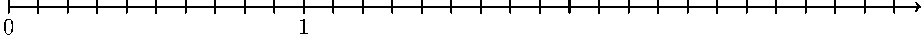
\includegraphics{tallin_0_3}
	\item Marker tala $ 1,1 $ og $ 2,5 $.\\[10pt]	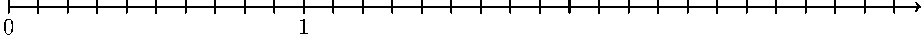
\includegraphics{tallin_0_3}
	\item Marker tala $ 0,4 $ og $ 3,0 $.\\[10pt]	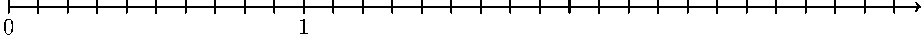
\includegraphics{tallin_0_3}
	\item Marker tala $ 1,9 $ og $ 2,9 $.\\[10pt]	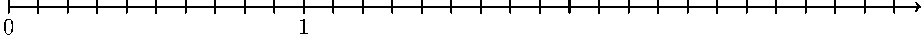
\includegraphics{tallin_0_3}
	\item Marker tala $ 1,2 $ og $ 2,5 $.\\[10pt]	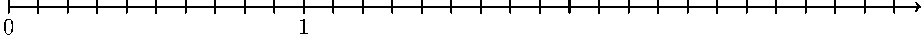
\includegraphics{tallin_0_3}
	
\end{enumerate}

\newpage
\pagestyle{empty}

\end{document}